\documentclass[12pt]{article}
    \usepackage{amsthm,amsmath,amssymb}
    \usepackage{amsfonts}
    \usepackage{mathrsfs}
    \usepackage{listings}
    \usepackage{verbatim}
    \usepackage{fancyhdr}
    \usepackage{graphicx}
    \usepackage{xeCJK}
    \usepackage{xcolor}      %代码着色宏包
    \usepackage{CJK}         %显示中文宏包
    \usepackage{fontspec}
    \usepackage{float}
    \usepackage{placeins}
    \usepackage{subfigure}
    \usepackage{bm}
    \usepackage[colorlinks,linkcolor=blue]{hyperref}

\lstset{
    basicstyle=\fontspec{Consolas},
    %numbers=left,
    %rulesepcolor=\color{red!20!green!20!blue!20},
    escapeinside=``,
    xleftmargin=2em,xrightmargin=2em, aboveskip=1em,
    %背景框
    framexleftmargin=1.5mm,
    frame=shadowbox,
    %背景色
    backgroundcolor=\color[RGB]{245,245,244},
    %样式
    keywordstyle=\color{blue}\fontspec{Consolas Bold},
    %identifierstyle=\bf,
	breaklines=true,
    numberstyle=\color[RGB]{0,192,192},
    commentstyle=\color[RGB]{96,96,96}\fontspec{Consolas Italic},
    stringstyle=\rmfamily\slshape\color[RGB]{128,0,0},
    %显示空格
    showstringspaces=false
}

\textheight 23cm \textwidth 15cm
\topmargin -1.5cm \oddsidemargin 0.3cm \evensidemargin -0.3cm

\begin{document}
\title {Assignment-matlab 2}
\date{\today}
\author{Haowei Kan}
\maketitle
\section{Introduction}
Image editing tasks concern either global changes or local changes confined to a selection. Here we are interested in achieving local changes. With classic tools to achieve that, changes in the selected regions result in visible seams.

In this experiment, we will introduce a generic interpolation machinery based on solving Poisson equations, and a cloning tool, which is an application of this machinery for seamless editing of image regions will be shown.

\section{Algorithm}
\subsection{Generic machinery}
We know that slow gradients of intensity can be superimposed on an image with barely noticeable effect, and a scalar function on a bounded domain is uniquely defined by its values on the boundary and its Laplacian in the interior. So, given methods for crafting the Laplacian of an unknown function over some domain, and its boudary conditions, the Poisson equation can be solved numerically to achieve seamless filling of that domain. When applied to the image editting, it can be replicated independently in each of the channels of a color image.

Solving the Poisson equation also has an alternative interpretation as a minimization problem: it computes the function whose gradient is the closest, in the $L_2$-norm, to some prescribed vector field -- the $guidance$ vector field -- under given boundary conditions inwards, while following the spatial variations of the guidance filed as closely as possible.
\subsection{Discrete Poisson solver}
For discrete images, the problem can be discretized naturally using the underlying discrete pixel grid. Let S be the set of all the pixels of an image, $\Omega$ be a subset of S with boundary $\partial\Omega$. For each pixel p in S, let $N_p$ be the set of its 4-connected neighbors which are in S, and let $\langle p,q\rangle$ denote a pixel pair s.t. $q\in N_p$. The boundary of $\Omega$ is now $\partial\Omega=\left\{p\in S\setminus\Omega:N_p\cap\Omega\neq\emptyset\right\}$. Let $f_p$ be the value of $f$ at $p$. The task is to compute the set of intensities $f|_\Omega=\left\{f_p,p\in\Omega\right\}$.

Then the discrete optimization problem will be:
\begin{equation}
    \min_{f|_\Omega}\sum_{\langle p,q\rangle\cap\Omega\neq\emptyset}(f_p-f_q-v_{pq})^2,\  \mathrm{with}\ f_p=f_p^*,\mathrm{\ for\  all\  p}\in\partial\Omega
\end{equation}
where $v_{pq}$ can be thought as the guided vector field in discrete problem.

Its solution satisfies the following simultaneous linear equations:
\begin{equation}
    \mathrm{for\ all}\ p\in\Omega,\ |N_p|f_p-\sum_{q\in N_p\cap\Omega}f_q=\sum_{q\in N_p\cap\partial\Omega}f_q^*+\sum_{q\in N_p}v_{pq}
\end{equation}
So we can calculate unknown values $f_p$ on $\Omega$ by solving these linear equations.
\subsection{Mixed seamless cloning}
To apply the Poisson image editting to seamless cloning, we can think the each channel of destinated area on the background is the unknown set $\Omega$ that need to be computed by discrete poisson solver. And the $v_{pq}$ is related to the cloning area taken from source image.

So all we need to determine for the linear equations is the values of $v_{pq}$. In this experiment, we choose the mixing gradients to solve the problem, which is
\begin{equation}
    v_{pq}=\left\{
    \begin{array}{cc}
        f^*_p-f^*_q & \ \ \ \ \mathrm{if}\ |f^*_p-f^*_q|>|g_p-g_q| \\
        g_p-g_q     & \mathrm{otherwise}
    \end{array}
    \right.
\end{equation}
for all $\langle p,q\rangle$, where $g_p$ is the value of pixel $p$ in source image.
\subsection{Real-time cloning}
In this experiment, we are required to acheive real-time cloning when moving the destinated area on background. Therefore, we need to consider decreasing the runtime of our algorithm. Notice that the coefficient matrix will be unchanged when moving the destinated area if we don't drag it out of the background. So we can store the coefficient matrix and reuse it in real-time computation. Here are some further measures we took:
\begin{enumerate}
    \item use the sparse matrix to store the coefficients of the linear equations
    \item pre-decomposite the coefficient matrix through Cholesky method
\end{enumerate}

\section{Result}
\begin{figure}[H]
    \subfigure[source image]{
        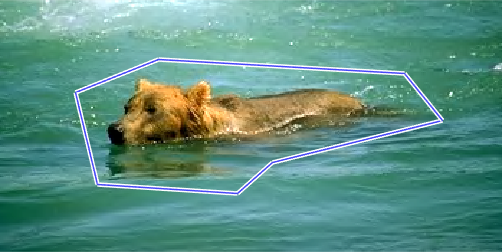
\includegraphics[width=0.5\textwidth]{result/1.png}
    }
    \subfigure[mixed seamless cloning 1]{
        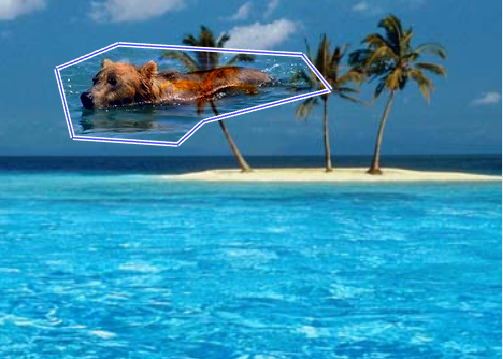
\includegraphics[width=0.5\textwidth]{result/2.png}
    }
    \subfigure[mixed seamless cloning 2]{
        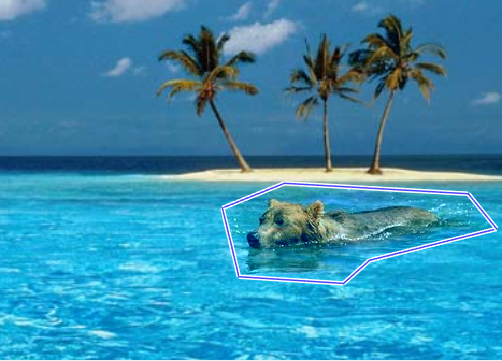
\includegraphics[width=0.5\textwidth]{result/3.png}
    }
    \subfigure[mixed seamless cloning 3]{
        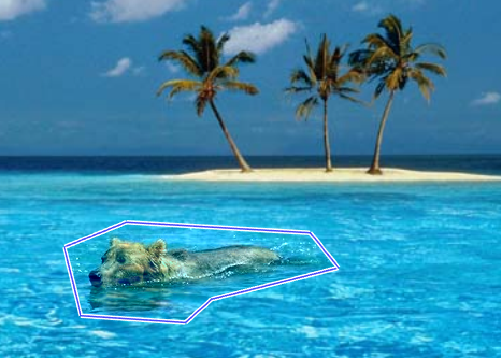
\includegraphics[width=0.5\textwidth]{result/4.png}
    }

\end{figure}
\section{Why Cholesky method}
Notice that the coefficient matrix we get is a real symmetrix positive definite matrix. So the Cholesky method is the best choice. And here is a table of the range of runtime of LU, QR and Cholesky method for a 15845$\times$15845 sparse matrix in our real-time calculation.
\begin{table}[htb]
    \centering
    \begin{tabular}{|c|c|c|c|}
        \hline
        method             & LU             & QR             & Chol           \\
        \hline
        range of runtim(s) & (0.008, 0.011) & (0.019, 0.022) & (0.004, 0.006) \\
        \hline
    \end{tabular}
\end{table}

This verifies that Cholesky method for this problem gives the best performance.

\newpage
\appendix
\section{Code}
All the code of this assignment can be downloaded from \url{https://github.com/mathendy/MS-USTC/tree/master/Code%20Training/matlab-2_assignment}

\end{document}